\documentclass[10pt]{beamer}
%for(int i=0; i<n; i++){\documentclass[10pt,handout]{beamer}
\usepackage[spanish]{babel}
% % \usepackage[backend=biber, style=authoryear-icomp]{biblatex}
\resetcounteronoverlays{exx}
\usepackage{mdframed}
\usepackage{tikz}
\usepackage{blindtext}
\usepackage{tipa}
% \usepackage{cgloss4e}
% \usepackage{gb4e}
% \usepackage{qtree}
\usepackage{cancel}
\usepackage{wrapfig}
\usepackage{soul}
\usepackage{enumerate}
\usepackage{longtable}
\graphicspath{ {./figures/} } % declaramos donde estan las imagenes
\usepackage[labelformat=simple]{subcaption} % para varias imagenes juntas
\renewcommand\thesubfigure{(\alph{subfigure})}
\usepackage[utf8]{inputenc}
\usepackage{amsmath}
\usepackage{amsfonts} % simbolos como el I de matriz identidad
\usepackage{bm}
\usepackage{graphicx} % paquete para ver imagenes
\usepackage{setspace}
\usepackage[T1]{fontenc}
\usepackage{parskip}
\usepackage{color}
\usepackage{framed}

\usetheme{Copenhagen}
\definecolor{frenchblue}{rgb}{0.0, 0.45, 0.73} % ESTE!!!!

\setbeamercolor{block body}{bg=frenchblue!50}
\setbeamercolor*{structure}{fg=frenchblue,bg=blue}
\setbeamercolor{normal text}{fg=black}
\setbeamercolor{frametitle}{bg=black}
\setbeamertemplate{frametitle}[default][center]
\setlength{\parskip}{12pt}
\useoutertheme{infolines} % me comia mucho espacio de la otra fgorma
\makeatother
\setbeamertemplate{footline}
{
  \leavevmode%
  \hbox{%
  \begin{beamercolorbox}[wd=.3\paperwidth,ht=2.25ex,dp=1ex,center]{author in head/foot}%
    \usebeamerfont{author in head/foot}\insertshortauthor
  \end{beamercolorbox}%
  \begin{beamercolorbox}[wd=.6\paperwidth,ht=2.25ex,dp=1ex,center]{title in head/foot}%
    \usebeamerfont{title in head/foot}\insertshorttitle
  \end{beamercolorbox}%
  \begin{beamercolorbox}[wd=.1\paperwidth,ht=2.25ex,dp=1ex,center]{date in head/foot}%
    \insertframenumber{} / \inserttotalframenumber\hspace*{1ex}
  \end{beamercolorbox}}%
  \vskip0pt%
}
\makeatletter
\setbeamertemplate{navigation symbols}{}
%\setbeameroption{show notes}
\setbeameroption{hide notes}
\renewcommand{\CancelColor}{\color{red}}

\usepackage{hyperref}

\title[Flip-Flop JK]{Organizaci\'on del Computador I: Flip-Flop JK}
\author[Matias Mazzanti]{Matias Mazzanti}


\institute{DC-UBA}
\date{09 de Agosto de 2022}

\titlegraphic{
\includegraphics[,height=2cm,keepaspectratio]{../../logo.pdf}     }
%\logo{
\includegraphics[height=2.5cm]{logo.PDF}}

\begin{document}

\begin{frame}

\maketitle

\end{frame}


\section{Presentaci\'on}
\begin{frame}
\frametitle{Introducción}
\begin{mdframed}[backgroundcolor=frenchblue!20]
  Tema del día: Flip-Flops JK
\end{mdframed}

\begin{itemize}
  \item Repaso.
  \item Definición.
  \item Motivación.
  \item Ejercicio.
  \item Solución.
  \item Conclusiones.
\end{itemize}

\end{frame}
\begin{frame}
\frametitle{Repaso}
En donde estábamos?

Circuitos \textbf{Combinacionales}: La salida  esta determinada únicamente por la entrada
del circuito.

Circuitos \textbf{Secuenciales}: La salida esta determinada por la entrada y por el \textbf{estado}
del circuito.
\begin{columns}
    \column{0.5\textwidth}

Estos los podemos pensar como un bloque combinacional y un bloque con memoria.

Donde E es la entrada S es la salida y  Q$_n$ el estado de la memoria en tiempo $n$.
    \column{0.5\textwidth}
        \begin{figure}[h!]
    \centering
    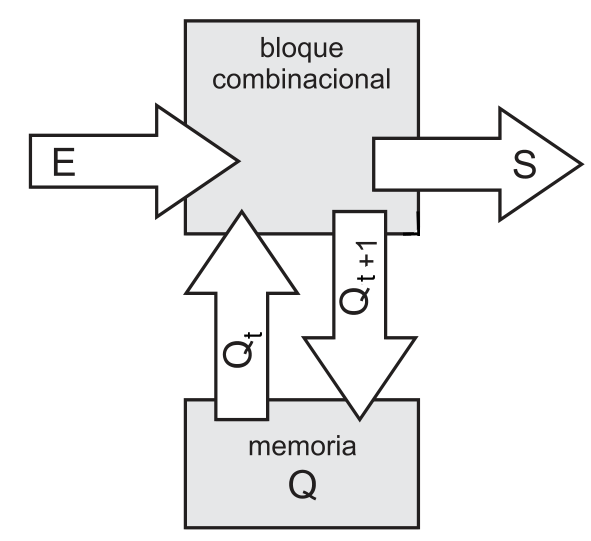
\includegraphics[scale=0.2]{secuencial.png}
\end{figure}
\end{columns}

\end{frame}

\begin{frame}
\frametitle{Repaso}

\begin{columns}
    \column{0.5\textwidth}
        Vimos que al intentar almacenar un bit de la forma trivial: un OR o AND.

El circuito se traba.

\vspace{1cm}

Luego de almacenar un valor, no puedo cambiarlo.
\vspace{1cm}

Ademas me interesa tener control sobre cuando podemos cambiar el valor almacenado!

Se\~nal de clock!


    \column{0.5\textwidth}
        \begin{figure}[h!]
            \centering
            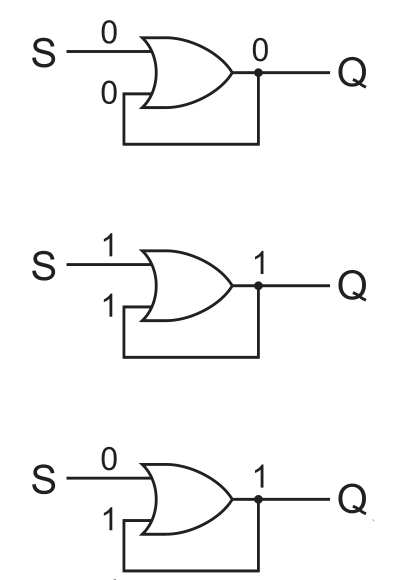
\includegraphics[scale=0.3]{unbit.png}
        \end{figure}
\end{columns}
\end{frame}

\begin{frame}
\frametitle{Repaso}
\begin{mdframed}[backgroundcolor=frenchblue!20]
  El Flip-Flop resuelve este problema con m\'as de un componente y con retroalimentaci\'on.
\end{mdframed}
\vspace{0.2cm}
\begin{columns}
      \column{0.5\textwidth}
        Flip-Flops RS: Reset and Set

         \begin{figure}[h!]
             \centering
             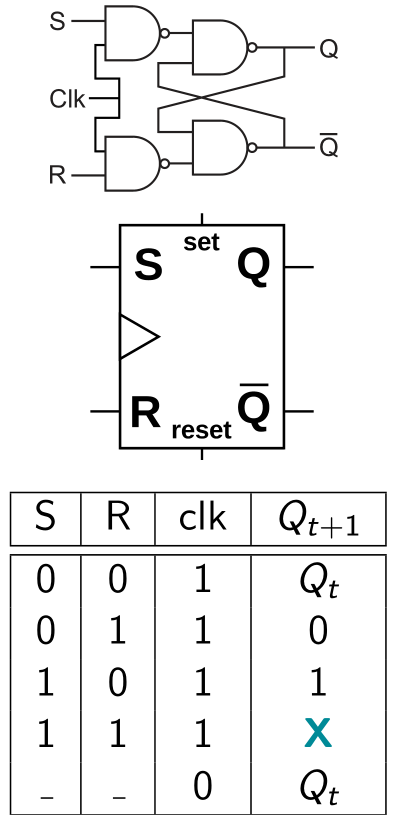
\includegraphics[scale=0.18]{flipRS.png}
         \end{figure}
    \column{0.5\textwidth}
        Flip-Flops D: Delay

\begin{figure}[h!]
    \centering
    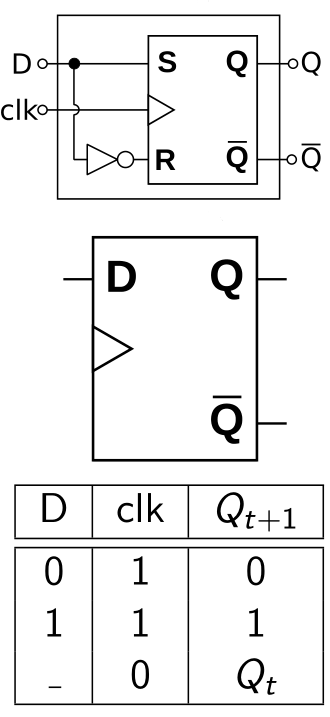
\includegraphics[scale=0.18]{flipD.png}
\end{figure}


\end{columns}

\end{frame}



\begin{frame}
\frametitle{Flip-Flop JK}
Flip-Flop JK resuelve el problema del input R=1 y S=1 del RS.

Ademas aprovecha el delay para generar cambios solo en los flancos de la se\~nal de clock.

Lo realiza con un \textbf{detector de pulsos}. Circuito AND, único input duplicado,  negando una de las entradas.
\begin{figure}[h!]
    \centering
    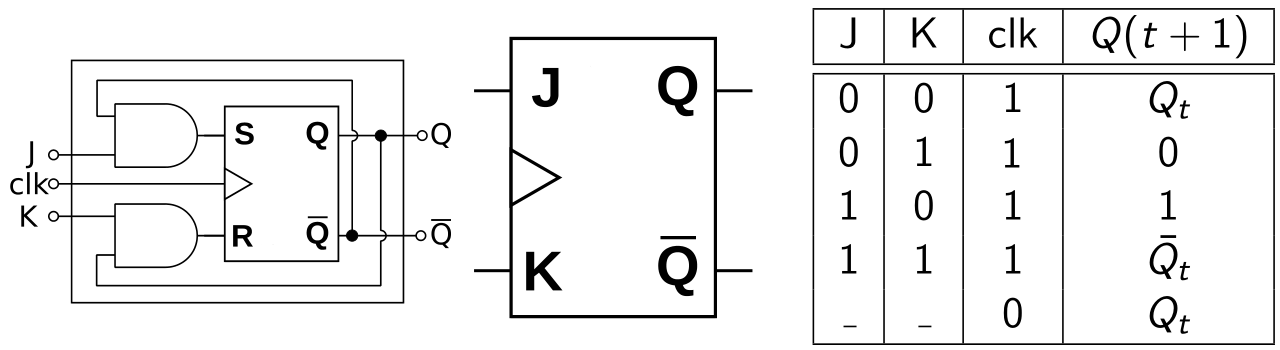
\includegraphics[scale=0.2]{flipJK.png}
\end{figure}



\end{frame}
\begin{frame}
\frametitle{Motivación}

Al poder dominar el almacenamiento de un bit de forma controlada, permite poder construir
cualquier tipo de almacenamiento.

No necesariamente las memorias modernas utilizan esta tecnología.

Bloque fundamental de las  FPGA.

\begin{figure}[h!]
    \centering
    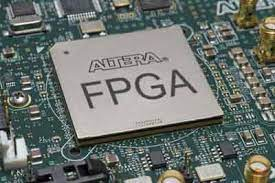
\includegraphics[scale=0.5]{fpga.jpeg}
\end{figure}
\end{frame}


\begin{frame}
\frametitle{Ejercicio}

Implementar un registro de dos bits que siga los siguientes estados
y que cada cambio se produzca al apretar un pulsador. Usando
flip-flops JK y compuertas b\'asicas a elecci\'on.
Nos piden adem\'as que el componente a desarrollar cuente con una
entrada de Reset.

\begin{figure}[h!]
    \centering
    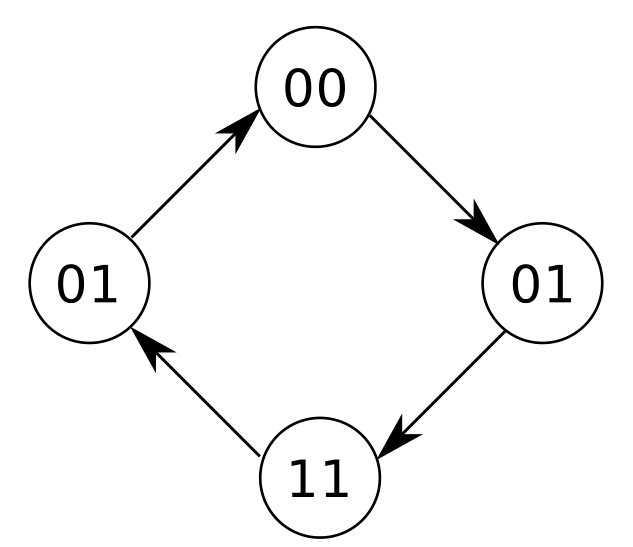
\includegraphics[scale=0.21]{ej1.png}
\end{figure}
\end{frame}

\begin{frame}
\frametitle{Solución}

En principio.... ? Como arrancamos?

\begin{mdframed}[backgroundcolor=frenchblue!20]
  TABLAS DE VERDAD!
\end{mdframed}
\only<1>{\begin{table}[h!]
\begin{tabular}{|c|c|c|c|c|}
\hline
Q$_0$(t) & Q$_1$(t) &  & Q$_0$(t+1) & Q$_1$(t+1) \\ \hline
0        & 0        &  &           &          \\ \hline
0        & 1        &  &           &           \\ \hline
1        & 0        &  &           &           \\ \hline
1        & 1        &  &          &           \\ \hline
\end{tabular}
\end{table}}
\only<2>{\begin{table}[h!]
\begin{tabular}{|c|c|c|c|c|}
\hline
Q$_0$(t) & Q$_1$(t) &  & Q$_0$(t+1) & Q$_1$(t+1) \\ \hline
0        & 0        &  & 0          & 1          \\ \hline
0        & 1        &  &           &           \\ \hline
1        & 0        &  &           &           \\ \hline
1        & 1        &  &          &           \\ \hline
\end{tabular}
\end{table}}
\only<3>{\begin{table}[h!]
\begin{tabular}{|c|c|c|c|c|}
\hline
Q$_0$(t) & Q$_1$(t) &  & Q$_0$(t+1) & Q$_1$(t+1) \\ \hline
0        & 0        &  & 0          & 1          \\ \hline
0        & 1        &  & 1          & 0          \\ \hline
1        & 0        &  &           &          \\ \hline
1        & 1        &  &           &           \\ \hline
\end{tabular}
\end{table}}
\only<4>{\begin{table}[h!]
\begin{tabular}{|c|c|c|c|c|}
\hline
Q$_0$(t) & Q$_1$(t) &  & Q$_0$(t+1) & Q$_1$(t+1) \\ \hline
0        & 0        &  & 0          & 1          \\ \hline
0        & 1        &  & 1          & 0          \\ \hline
1        & 0        &  & 1          & 1          \\ \hline
1        & 1        &  &           &           \\ \hline
\end{tabular}
\end{table}}
\only<5>{\begin{table}[h!]
\begin{tabular}{|c|c|c|c|c|}
\hline
Q$_0$(t) & Q$_1$(t) &  & Q$_0$(t+1) & Q$_1$(t+1) \\ \hline
0        & 0        &  & 0          & 1          \\ \hline
0        & 1        &  & 1          & 0          \\ \hline
1        & 0        &  & 1          & 1          \\ \hline
1        & 1        &  & 0          & 0          \\ \hline
\end{tabular}
\end{table}}
Esto es lo que quiero, y ahora?
\end{frame}


\begin{frame}
\frametitle{Solución}

\begin{figure}[h!]
    \centering
    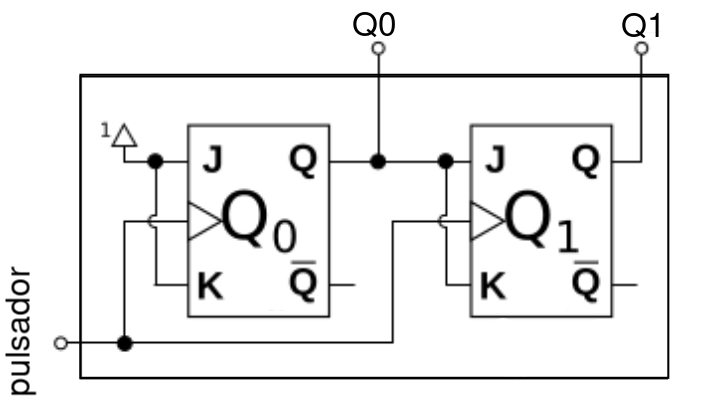
\includegraphics[scale=0.2]{circuito.png}
\end{figure}
\end{frame}

\end{document}
